% enable this to activate the version for PRINT
% disable this to make the pdf symmetric and without white pages
% => asymmetric alternating left/right margins
% \newcommand*{\printversion}{}%

%% | ---------------- document meta information --------------- |

\newcommand{\Author}{Tadeáš Zribko}
\newcommand{\Department}{Department of Computer Science}
\newcommand{\Supervisor}{Ing. Karel Frajták, Ph.D.}
\newcommand{\SupervisorSpecialist}{Ing. My Specialist, Ph.D.}
\newcommand{\Programme}{Open informatics}
\newcommand{\Field}{Software Engineering}
\newcommand{\Title}{NUnit test framework extension for\\[0.5em]test data preparation}
\newcommand{\Keywords}{}
\newcommand{\KlicovaSlova}{}
\newcommand{\Year}{2025}
\newcommand{\Month}{May}
\newcommand{\Date}{\Month~\Year}
\newcommand{\Location}{Prague}

%% | ---------------------- configuration --------------------- |

% most of the configuration stuff happens here
%!TEX root = ../main.tex

%% | ----------------------- page setup ----------------------- |

% define documentclass based on the print/screen version of the document
\pdfoutput=1
\ifdefined\printversion
  \documentclass[a4paper,11pt,twoside,openright]{book}
\else
  \documentclass[a4paper,11pt,twoside,openany]{book}
\fi

% define how "clearpage" works with the print/screen version of the document
\newcommand{\conditionalClearPage}{
  \ifdefined\printversion
    \cleardoublepage
  \else
    \clearpage
  \fi
}

%% | ----------------- commonly used packages ----------------- |

\usepackage[english]{babel}
\usepackage{csquotes}
\usepackage{amsmath,amsfonts,amssymb,bm}
\usepackage{nicefrac}
\usepackage{algorithm,algpseudocode}
\usepackage[title,titletoc]{appendix}
\usepackage{latexsym}
\usepackage{a4wide}
\usepackage{color}
\usepackage{indentfirst}
\usepackage{graphicx}
\usepackage{fancyhdr,lastpage}
\usepackage{longtable}
\usepackage{pifont}
\usepackage{makeidx}
\usepackage{multirow}
\usepackage{dcolumn}
\usepackage{epstopdf}
\usepackage{url}
\usepackage{listings}
\usepackage{relsize}
\usepackage{pdfpages}
\usepackage{url}
\usepackage{lipsum}
\usepackage{isotope}
\usepackage{verbatim}
\usepackage{xcolor}
\usepackage{tcolorbox}
\usepackage[colorlinks]{hyperref}
\usepackage{multicol}
\usepackage{subfig}
\usepackage[export]{adjustbox}

% print version has different margins to accommodate the spine of the book
% do not move this around, or it stops working
\ifdefined\printversion
  \usepackage[a4paper,margin=3.2cm,inner=3.4cm,outer=2.0cm]{geometry}
\else
  \usepackage[a4paper,margin=3.2cm,inner=2.7cm,outer=2.7cm]{geometry}
\fi

\hyphenation{}

%% | --------------------- custom commands -------------------- |

\definecolor{cvutblue}{cmyk}{1, 0.43, 0, 0}

% set itemize: bullets type and color
\renewcommand{\labelitemi}{\textcolor{cvutblue}{\raisebox{.45ex}{\rule{.8ex}{.8ex}}}}
\renewcommand{\labelitemii}{\textcolor{cvutblue}{\raisebox{.45ex}{\rule{.8ex}{.8ex}}}}
\renewcommand{\labelitemiii}{\textcolor{cvutblue}{\raisebox{.45ex}{\rule{.8ex}{.8ex}}}}
\renewcommand{\labelitemiv}{\textcolor{cvutblue}{\raisebox{.45ex}{\rule{.8ex}{.8ex}}}}


%% | ---------------------- abbreviations --------------------- |

\usepackage[printonlyused]{acronym}

% use to change margins around abbreviations block
\def\changemargin#1#2{\list{}{\rightmargin#2\leftmargin#1}\item[]}
\let\endchangemargin=\endlist

%% | -------------------- hyper links setup ------------------- |
\hypersetup{
  linkcolor=black,
  anchorcolor=black,
  citecolor=cvutblue,
  filecolor=black,
  menucolor=black,
  runcolor=black,
  urlcolor=cvutblue
}


%% | -------------------------- tikz -------------------------- |

\usepackage{tikz}
\usepackage{pgfplots}
\pgfplotsset{compat=1.14}
\usetikzlibrary{backgrounds,arrows,automata,shapes,positioning,calc,through,spy,shapes,shapes.geometric,shapes.multipart,fit,patterns,fadings}
\pgfdeclarelayer{background}
\pgfdeclarelayer{foreground}
\pgfsetlayers{background,main,foreground}

%% | ------------ siunitx for units of measurements ----------- |

\usepackage{siunitx}
\DeclareSIUnit \parsec {pc}
\DeclareSIUnit \electronvolt {eV}
\DeclareSIUnit \pixel {px}
\DeclareSIUnit \arcmin {arcmin}
\DeclareSIUnit \erg {erg}
\DeclareSIUnit \joul {J}

%% | --------------- change formatting of lists --------------- |

\usepackage{enumitem}
\setlist{nosep}

\renewcommand{\labelenumi}{(\roman{enumi})}

%% | -------------------- table of contents ------------------- |

\usepackage[subfigure]{tocloft}

\tocloftpagestyle{plain}

%% | ----------------- formatting of a chapter ---------------- |

\usepackage{titlesec}

\titleformat{\chapter}[hang]{}{\color{cvutblue}\rule[-0.03cm]{0.50cm}{0.50cm}}{3.2\parskip}{\normalfont\bfseries\LARGE\thechapter\hspace{0.5cm}}
\titlespacing*{\chapter}{0pt}{-1em}{1.5em}

%% | ----------------- formatting of a section ---------------- |

\titleformat{\section}[hang]{}{\hspace{0.11cm}\color{cvutblue}\rule[-0.02cm]{0.30cm}{0.30cm}}{3.7\parskip}{\normalfont\bfseries\large\thesection\hspace{0.5cm}}
\titlespacing*{\section}{0pt}{1em}{0.5em}

\titleformat{name=\section,numberless}[block]
{\normalfont\large\bfseries}{}{0pt}{\large}
% {?}{before}{after}
\titlespacing*{name=\section,numberless}{0pt}{-1em}{2em}

%% | --------------- formatting of a subsection --------------- |

\titleformat{\subsection}[hang]{}{\hspace{0.16cm}\color{cvutblue}\rule[0.03cm]{0.20cm}{0.20cm}}{4.0\parskip}{\normalfont\bfseries\normalsize}
\titlespacing*{\subsection}{0pt}{1em}{0.5em}



%% | ------------------------ biblatex ------------------------ |

\usepackage[backend=bibtex,defernumbers=true,style=ieee,sorting=ydnt,sortcites=true]{biblatex}

% define the source file with bibliography
\addbibresource{main.bib}

\renewcommand*{\bibfont}{\Font}

% add suffix "a" to publications containing the keyword "mine"
% add suffix "c" to publications containing the keyword "mine" && "core"
\DeclareFieldFormat{labelnumber}{%
  \ifkeyword{mine}
    {\ifkeyword{core}
      {{\number\numexpr#1}c}%
      {{\number\numexpr#1}a}%
    }%
    {#1}%
}

\DeclareCiteCommand{\tabcite}%[\mkbibbrackets]
  {\usebibmacro{cite:init}%
   \usebibmacro{prenote}}
  {\usebibmacro{citeindex}%
   \usebibmacro{cite:comp}}
  {}
  {\usebibmacro{cite:dump}%
   \usebibmacro{postnote}}

% define fullciteinbox command
\definecolor{light-gray}{gray}{0.95}
\newcommand{\fullciteinbox}[2]{%

\DeclareCiteCommand{\fullcite}
{\usebibmacro{prenote}}
{\clearfield{addendum}%
  \usedriver
  {\defcounter{minnames}{6}%
  \defcounter{maxnames}{6}}
{\thefield{entrytype}}}
{\multicitedelim}
{\usebibmacro{postnote}}

\begin{tcolorbox}[opacityfill=0.05,width=\textwidth,colback={cvutblue},colframe={cvutblue},title={}]%
\ifx&#2&
\else
  \textbf{#2}:\\\\
\fi
\begin{minipage}[t]{0.07\linewidth}%
\raggedright%
\cite{#1}%
\end{minipage}%
\begin{minipage}[t]{0.93\linewidth}%
\fullcite{#1}%
\end{minipage}%
\end{tcolorbox}%
%}%
\vspace{-0.3em}
}%

% change the bibliography font style
% does not compile without this
\let\bibfont\small

% this is used to print citations of author's work
\defbibenvironment{mycitations}
{\itemize}
{\enditemize}
{\item}

%% | ---------------------- custom macros --------------------- |

\newcommand{\strong}[1]{\textbf{#1}}
\newcommand{\coord}[1]{\textbf{#1}}
\newcommand{\norm}[1]{\left\lvert#1\right\rvert}
\newcommand{\m}[1]{\ensuremath{\mathbf{#1}}}
\newcommand\numberthis{\addtocounter{equation}{1}\tag{\theequation}}
\newcommand{\add}[1]{{\color{green} {#1}}}
\newcommand{\todo}[1]{{\color{red} TODO {#1}}}
\newcommand{\updated}[1]{{\color{blue} {#1}}}
\newcommand{\real}{\mathbb{R}}
\newcommand{\red}[1]{{\color{red} #1}}
\newcommand{\minus}{\scalebox{0.75}[1.0]{$-$}}
\newcommand{\plus}{\scalebox{0.8}[0.8]{$+$}}
\newcommand{\figvspace}{\vspace{-1em}}

% referencing
\newcommand{\reffig}[1]{Fig.~\ref{#1}}
\newcommand{\reflst}[1]{Lst.~\ref{#1}}
\newcommand{\refalg}[1]{Alg.~\ref{#1}}
\newcommand{\refsec}[1]{Sec.~\ref{#1}}
\newcommand{\reftab}[1]{Table~\ref{#1}}
\newcommand{\refeq}[1]{\eqref{#1}}

%% | ----------------- listings - showing code ---------------- |

\usepackage{listings}     
\usepackage{lstautogobble}  % Fix relative indenting
\usepackage{color}          % Code coloring
\usepackage{zi4}            % Nice font

\definecolor{bluekeywords}{rgb}{0.13, 0.13, 1}
\definecolor{greencomments}{rgb}{0, 0.5, 0}
\definecolor{redstrings}{rgb}{0.9, 0, 0}
\definecolor{graynumbers}{rgb}{0.5, 0.5, 0.5}

\usepackage{listings}
\lstset{
    autogobble,
    columns=fullflexible,
    showspaces=false,
    showtabs=false,
    breaklines=true,
    showstringspaces=false,
    breakatwhitespace=true,
    escapeinside={(*@}{@*)},
    commentstyle=\color{greencomments},
    keywordstyle=\color{bluekeywords},
    stringstyle=\color{redstrings},
    numberstyle=\color{graynumbers},
    basicstyle=\ttfamily\footnotesize,
    frame=l,
    framesep=12pt,
    xleftmargin=12pt,
    tabsize=4,
    captionpos=b
}

%% | -------------------- layout parameters ------------------- |

% no indent, free space between paragraphs
\setlength{\parindent}{1cm}
\setlength{\parskip}{1ex plus 0.5ex minus 0.2ex}

% offsets the head down
\setlength{\headheight}{18pt}

% foot line
\renewcommand{\footrulewidth}{0.4pt}

%% | -------------- define the 'full' page style -------------- |

\fancypagestyle{full}{%

  % clear the default layout
  \fancyhead{}
  \fancyfoot{}

  % page header
  \fancyhead[LO]{\leftmark}
  \fancyhead[RE]{\rightmark}
  \fancyhead[LE,RO]{\thepage/\pageref{LastPage}}

  % page footer
  \fancyfoot[L]{CTU in Prague}
  \fancyfoot[R]{\Department}
  \fancyfoot[C]{}
}

%% | -------------- define the 'plain' page style ------------- |

\fancypagestyle{plain}{%

  % clear the default layout
  \fancyhead{}
  \fancyfoot{}

  % page header
  \fancyhead[LE,RO]{\thepage}
}

%% | -------------- Adjust style of chapter names ------------- |

\renewcommand{\chaptermark}[1]{\markboth{\MakeUppercase{\thechapter.\ #1}}{}}

%% | -------- European layout, no extra space after '.' ------- |

\frenchspacing

%% | ----------- adjust the style of the first page ----------- |

\makeatletter
\renewcommand\chapter{\if@openright\cleardoublepage\else\clearpage\fi
                    \thispagestyle{full}% original style: plain
                    \global\@topnum\z@
                    \@afterindentfalse
                    \secdef\@chapter\@schapter}
\makeatother


%% | ---------------------- the contents ---------------------- |

\begin{document}

% this will prevent unwanted line overflows
% http://latexref.xyz/_005cfussy-_0026-_005csloppy.html
\sloppy

\pagenumbering{roman}




%% --------------------------------------------------------------
%% |                         Title page                         |
%% --------------------------------------------------------------

%!TEX root = ../main.tex

\begin{titlepage}
  \begin{center}

    \textsc{\Large Czech Technical University in Prague}\\[1em]
    \textsc{\large Faculty of Electrical Engineering\\
    \Department\\
    [3em]
    }
    
\includegraphics[height=4.1cm]{fig/ctu_lion.pdf}\\[3em]

    \textbf{\textsc{\Huge \Title}}\\[2em]

    \textbf{\Large Master's Thesis}\\[6em]

    \textbf{\huge \Author}\\[6em]

    {\large \Location, \Date}\\[3em]

    Study programme: \Programme\\
    Branch of study: \Field\\[4em]

    \textbf{Supervisor: \Supervisor}\\

    \vspace{2pt}

  \end{center}
\end{titlepage}




%% --------------------------------------------------------------
%% |                       Acknowledgments                      |
%% --------------------------------------------------------------
\pagestyle{plain}
\setcounter{page}{1}
\conditionalClearPage
% set up the page style for the "intro" pages

%!TEX root = ../main.tex

\section*{Acknowledgments}

Firstly, I would like to express my gratitude to my supervisor.

\vspace{2.5cm}

%% --------------------------------------------------------------
%% |                         Assignment                         |
%% --------------------------------------------------------------

\conditionalClearPage

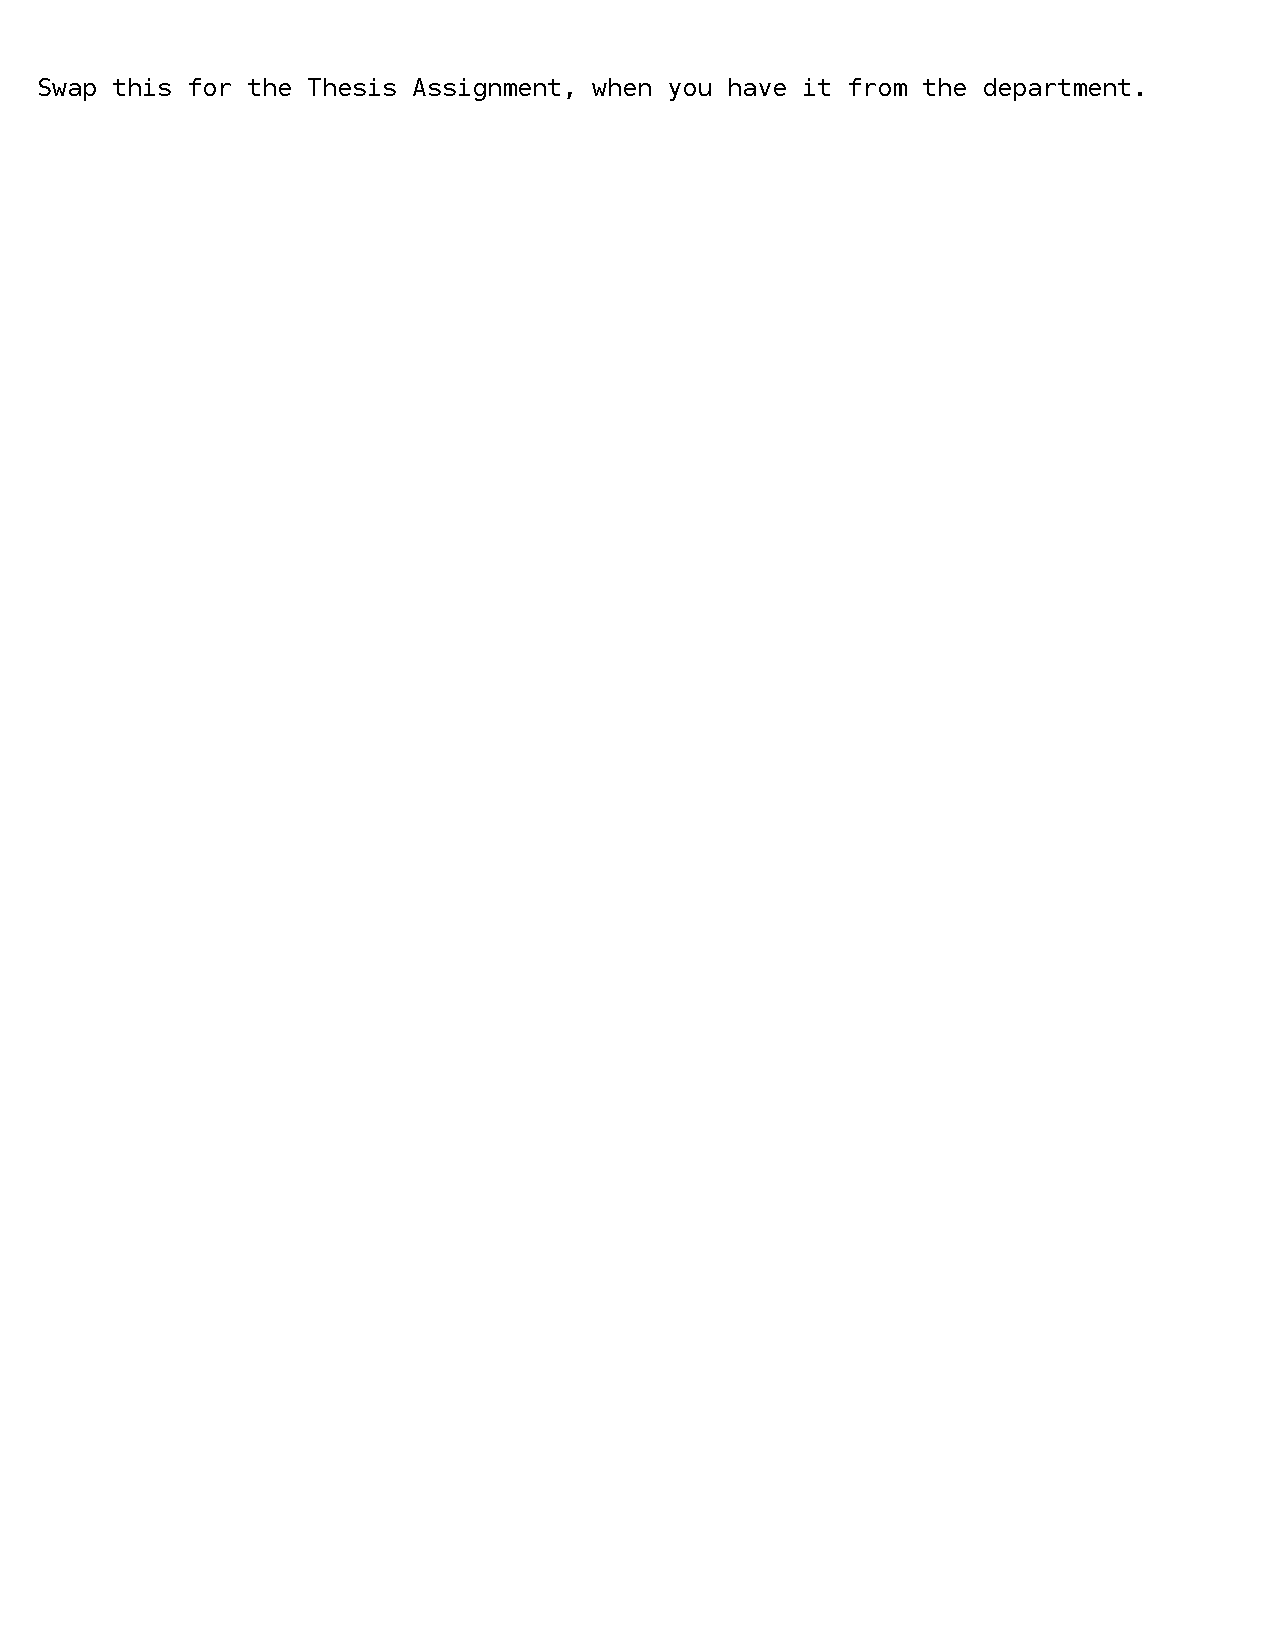
\includepdf{src/assignment.pdf}

%% --------------------------------------------------------------
%% |                         Declaration                        |
%% --------------------------------------------------------------

\conditionalClearPage

~\vfill{}

\section*{Declaration}
%\section*{Prohlášení autora práce}

I declare that presented work was developed independently, and that I have listed all sources of information used within, in accordance with the Methodical instructions for ob-serving ethical principles in preparation of university theses.
% Prohlašuji, že jsem předloženou práci vypracoval samostatně a že jsem uvedl veškeré použité informační zdroje v souladu s Metodickým pokynem o dodržování etických principů při přípravě vysokoškolských závěrečných prací.

\vspace{1.5cm}
~\\

Date .............................\hfill{}...............................................
% Dne.............................\hfill{}...............................................

\hfill{}~~~~~~~~~~~~~~~

\newpage{}


%% --------------------------------------------------------------
%% |                          Abstracts                         |
%% --------------------------------------------------------------

\conditionalClearPage

%!TEX root = ../main.tex

\begin{changemargin}{0.8cm}{0.8cm}

~\vfill{}

\section*{Abstract}
\vskip 0.5em

The study of autonomous \acp{UAV} has become a prominent sub-field of mobile robotics.

\vskip 1em

{\bf Keywords} \Keywords

\vskip 2.5cm

\end{changemargin}


\conditionalClearPage

v%!TEX root = ../main.tex

\begin{changemargin}{0.8cm}{0.8cm}

~\vfill{}

\section*{Abstrakt}
\vskip 0.5em

\sloppy
todo{}

\vskip 1em

{\bf Klíčová slova} \KlicovaSlova

\vskip 2.5cm

\end{changemargin}


%% --------------------------------------------------------------
%% |                        Abbreviations                       |
%% --------------------------------------------------------------

\conditionalClearPage

\begin{changemargin}{0.8cm}{0.8cm}

~\vfill{}

% this will print only the used abbreviations
%!TEX root = ../main.tex
\section*{Abbreviations}

\begin{acronym}
\acro{CTU}[CTU]{Czech Technical University}
\acro{BDD}[BDD]{Behavior-Driven Development}
\acro{BOA}[BOA]{Business Objective Action}
\acro{TDD}[TDD]{Test-Driven Development}
\acro{WPF}[WPF]{Windows Presentation Foundation}
\acro{WinUI}[WinUI]{Windows UI Library}
\acro{MAUI}[MAUI]{Multi-platform App UI}
\acro{CI/CT}[CI/CT]{Continuous Integration and Testing}
\acro{CI/CD}[CI/CD]{Continuous Integration and Continuous Delivery}
\acro{EF}[EF]{Entity Framework}
\acro{ORM}[ORM]{Object Relational Mapper}
\acro{DI}[DI]{Dependency Injection}

\acro{API}[API]{Application Programming Interface}
\acro{DOF}[DOF]{degree-of-freedom}
\acro{FOV}[FOV]{Field of View}
\acro{GNSS}[GNSS]{Global Navigation Satellite System}
\acro{GPS}[GPS]{Global Positioning System}
\acro{IMU}[IMU]{Inertial Measurement Unit}
\acro{LKF}[LKF]{Linear Kalman Filter}
\acro{LTI}[LTI]{Linear time-invariant}
\acro{LiDAR}[LiDAR]{Light Detection and Ranging}
\acro{MAV}[MAV]{Micro Aerial Vehicle}
\acro{MPC}[MPC]{Model Predictive Control}
\acro{MRS}[MRS]{Multi-robot Systems Group}
\acro{ROS}[ROS]{Robot Operating System}
\acro{RTK}[RTK]{Real-time Kinematics}
\acro{SLAM}[SLAM]{Simultaneous Localization And Mapping}
\acro{UAV}[UAV]{Unmanned Aerial Vehicle}
\acro{UGV}[UGV]{Unmanned Ground Vehicle}
\acro{UKF}[UKF]{Unscented Kalman Filter}

\end{acronym}


\vskip 2.5cm

\end{changemargin}

\conditionalClearPage

%% --------------------------------------------------------------
%% |                      Table of contents                     |
%% --------------------------------------------------------------

\tableofcontents

\conditionalClearPage

% set up the full page style with normal page numbering
\pagestyle{full}
\pagenumbering{arabic}

%% --------------------------------------------------------------
%% |                        introduction                        |
%% --------------------------------------------------------------
%!TEX root = ../main.tex

\chapter{Introduction\label{chap:introduction}}

...existing code...

\section{Motivation}

% Your motivation content here.

\section{Objectives}

% Your objectives content here.
%!TEX root = ../main.tex

\chapter{State of the Art\label{chap:state_of_the_art}}

...existing code...

\section{Current Software Testing Practices}

% Your content here.

\section{Existing Frameworks}

\subsection{IntelliTest Framework}

% Your content here.

\subsection{AutoFixture Framework}

% Your content here.

\section{Research Gaps}

% Your content here.
\chapter{Preliminaries\label{chap:preliminaries}}

The Preliminaries chapter serves as an introduction to the foundational concepts, tools, and methodologies that are relevant to the work presented in this work. This chapter provides a brief overview of the essential background information needed to understand the subsequent content, providing context for the more detailed discussions that follow. 

\section{Overview of C\#}

C\# is a static-typed, multi-paradigm language developed by Microsoft within the .NET framework. Initially launched in 2000, C\# was intended to provide the robustness and efficiency required for complex applications while maintaining simplicity and productivity. C\# architecture supports the development of scalable and maintainable software, ranging from standalone desktop applications to sophisticated web services and cloud-based systems.

The language distinguishes itself through features such as type safety, garbage collection, and comprehensive support for object-oriented principles. Furthermore, C\# integrates seamlessly with the .NET runtime, facilitating interoperability between multiple programming languages and platforms. The features of the C\# language make it a versatile and powerful tool in contemporary software development.

\subsection{The Role of Interfaces in C\#}

Interfaces\footnote{\href{https://learn.microsoft.com/en-us/dotnet/csharp/fundamentals/types/interfaces}{Interface definition by Microsoft}} are foundational constructs in C\# that specify a contract that defines a set of members, including methods, properties, events or indexers, without implementation details. The abstraction of the interface supports a decoupled design, allowing developers to clearly define the boundaries between components. Interfaces are central to object-oriented programming in C\#, enabling polymorphism and adhering to the substitution principle, where multiple implementations of an interface can be used interchangeably.

The use of interfaces in software design improves modularity and extensibility. For example, interfaces are often employed in API definitions, enabling cohesive interaction between disparate systems or components. A notable addition introduced in C\# .Net 8.0 is the ability of the interfaces to include default implementations, allowing developers to provide fundamental functionality without breaking backward compatibility. This feature highlights the language's ongoing evolution to meet modern programming needs.

\subsection{Attributes and Metadata in C\#}

The attributes\footnote{\href{https://learn.microsoft.com/en-us/dotnet/csharp/advanced-topics/reflection-and-attributes/}{Attributes definition by Microsoft}} in C\# are declarative constructs that allow developers to embed metadata within assemblies, classes, methods, and other elements of the program. The metadata provides supplementary information that can influence the behavior of a program during run-time or compile-time. Attributes are a key mechanism for declarative programming, allowing behaviors to be specified through annotations rather than imperative code.

The attributes serve various purposes. Built-in attributes, such as \texttt{[Serializable]} and \texttt{[Obsolete]}, simplify tasks by marking elements for serialization or flagging deprecated functionality. Custom attributes extend this capability, allowing developers to define domain-specific metadata. These custom attributes, implemented as classes derived from \texttt{System.Attribute}, support specialized use cases such as runtime validation or configuration of object-relational mappings.

The interaction between attributes and reflection in C\# is particularly notable. Reflection enables programmers to dynamically query and manipulate metadata, a feature widely used in frameworks like ASP.NET\footnote{ASP.NET is a framework for building dynamic, server-side web applications}, where attributes configure routing, data annotations, and other essential behaviors. Consequently, attributes are indispensable for building flexible and adaptive systems.

\subsection{Advanced Language Features}
In addition to interfaces and attributes, the C\# programming language includes a variety of sophisticated features that increase its expressiveness and functional efficiency:

\begin{itemize} 
\item \textbf{Generics:} Facilitate the creation of reusable and type-safe data structures and algorithms while maintaining high performance. 
\item \textbf{LINQ (Language Integrated Query):} Provides a declarative syntax for querying data collections, databases, and other sources, improving code clarity and reducing complexity. 
\item \textbf{Asynchronous Programming:} Enabled through the \texttt{async} and \texttt{await} keywords, simplifying the development of non-blocking and responsive applications. 
\item \textbf{Event-Driven Programming:} Supported by delegates and events, offering robust mechanisms for implementing observer patterns and managing asynchronous communication. \end{itemize}

These features demonstrate the flexibility and capability of C\#, equipping developers with tools to address a wide variety of programming challenges.

\subsection{Front-End Development with C\#}

C\# is predominantly recognized for its extensive application in back-end programming. However, its functionalities have been significantly broadened to encompass the front-end development arena, primarily due to the advent and implementation of frameworks such as Blazor, Forms, and Unity. These frameworks facilitate the construction of sophisticated user interfaces and interactive components, thereby enhancing the versatility and applicability of C\# in different development paradigms.

\subsubsection{Blazor for Web Development}  
Blazor allows developers to build web applications using C\# instead of JavaScript. Blazor supports both server-side and client-side execution, enabling interactive web applications with shared code between the client and the server.
\subsubsection{Cross-Platform Development with Xamarin.Forms and MAUI}  
Xamarin.Forms enables the creation of native user interfaces for iOS, Android, and Windows with a shared C\# codebase, supporting features such as custom renderers and the MVVM \footnote{Model-View-ViewModel, a software architectural pattern used for designing the structure of user interfaces, particularly in desktop and mobile applications.} pattern for easier app maintenance. 
Xamarin.Forms has evolved into \ac{MAUI}, representing an integral part of the next-generation cross-platform development framework provided by the .NET ecosystem. 
\ac{MAUI} extends the foundational work established by Xamarin.Forms by offering advanced functionalities, including support for an expanded range of platforms such as macOS and Linux. \ac{MAUI} serves as a comprehensive framework for developing cross-platform applications, minimizing the need for platform-specific code and improving the development experience. Through \ac{MAUI}, developers have the ability to compose a singular codebase for applications intended for mobile and desktop devices, utilizing the capabilities of C\# and .NET across all platforms.

\subsubsection{Desktop UI with WPF and WinUI}  
\ac{WPF} \footnote{Graphical subsystem for rendering user interfaces in Windows applications.} and \ac{WinUI} \footnote{Modern user interface framework for creating native Windows applications with advanced UI elements and better performance}are used to develop desktop applications in C\#. \ac{WPF} utilizes XAML \footnote{Extensible Application Markup Language} for the design of the user interface, while \ac{WinUI}  offers modern user interface elements and improved performance for Windows applications.

\subsubsection{Gaming with Unity}

Unity\footnote{\href{https://unity.com/}{https://unity.com/}} is a robust game development engine that employs C\# for scripting, facilitating the creation of 2D and 3D games. Unitu is equipped with capabilities for cross-platform deployment, allowing games to operate on iOS, Android, Windows, macOS, and gaming consoles. The engine furnishes tools for real-time rendering, physics simulations, and complex animations, rendering it exemplary for developing immersive and interactive game experiences. The component-based architecture of Unity enables developers to attach C\# scripts to game objects to regulate their behavior and interactions. Due to its comprehensive documentation and active community, Unity is favored as a platform for constructing games across diverse platforms.

\section{Factory Pattern in Software Design}\label{sec:FactoryPattern}
The Factory Pattern is a fundamental creation design pattern that encapsulates the instantiation logic of objects defined in \cite{Gamma1994}. Delegating the responsibility of their creation to a specialized factory class. This abstraction allows client code to remain decoupled from specific class implementations, thereby enhancing modularity and facilitating future modifications.

\subsection{Advantages of the Factory Pattern}
\begin{itemize} 
\item  Encapsulation of Object Creation: The pattern abstracts the instantiation process, mitigating direct dependencies between components and promoting loose coupling.
\item  Enhanced Code Maintainability: By centralizing object creation logic within a factory, modifications to class structures become more manageable and localized \cite{Martin2008Aug}.
\item Support for Dependency Injection: The pattern integrates seamlessly with dependency injection frameworks, fostering a more scalable and maintainable software architecture.
\end{itemize}

\section{Software Testing Concepts}

Software testing is a critical activity in the software development life cycle, with the aim of ensuring the correctness, quality, and performance of a software system. Software testing involves the execution of software to detect defects, assess its functionality, and validate that a software meets the specified requirements. Testing can be performed at various stages of the development process to identify issues early and prevent the introduction of defects into the system.

According to \cite{hooda2015software}, software testing is typically categorized into several distinct types, each focusing on different aspects of software behavior.

\begin{itemize}
    \item \textbf{Unit Testing:} This type of testing focuses on evaluating individual components or functions of the system in isolation. Unit tests ensure that each unit of code performs as expected, which helps to prevent errors at the earliest stages of development.
    \item \textbf{Integration Testing:} After individual components have been verified, integration testing ensures that multiple components or systems interact as intended. Verifies data flow, communication between modules, and the system behavior when various components are combined.
    \item \textbf{System Testing:} System testing involves testing the complete system as a whole, ensuring that all components work seamlessly. Validates the functionality of the entire software and the compliance with the defined requirements and specifications.
    \item \textbf{Acceptance Testing:} Acceptance Testing is carried out to verify whether the software meets the business requirements and expectations of the end users. Acceptance testing is often performed by users or representatives to determine if the system is ready for deployment.
    \item \textbf{Regression Testing:} Regression testing is performed after code changes, bug fixes, or enhancements to features. The primary purpose of regression testing is to ensure that new changes do not introduce unwanted side effects or break existing functionality in the system.
    \item \textbf{Performance Testing:} Performance testing evaluates the responsiveness, stability, and scalability of the system under varying loads. Performance testing includes load testing, stress testing, and scalability testing to identify potential performance bottlenecks and ensure the system performs efficiently under real-world conditions.
    \item \textbf{Black-Box Testing:} Black-box testing evaluates software functionality without considering its internal structure or implementation details. The testers provide input and assess the output to verify that the system behaves as expected.
    \item \textbf{White-Box Testing:} White-box testing involves examining the internal workings of an application, including code structure, logic, and flow. It requires knowledge of the internal design and is often used for unit testing and code coverage analysis.
\end{itemize}

The process of software testing is not limited to the detection of defects. When defects are identified during any phase of testing, a structured process is followed to diagnose, isolate, and correct the issue. The defect is typically logged in a defect tracking system, where it is categorized and prioritized based on its severity. The development team then analyzes the root cause of the issue, applies a solution, and re-initiates testing to confirm that the problem has been resolved and no new issues have emerged.

The development process is inherently iterative, particularly in agile environments. Once a defect is discovered, the system undergoes debugging, corrections, and another round of testing to ensure that the changes made do not negatively impact the overall system. The iterative process of detection, diagnosis, resolution, and validation contributes to the continuous improvement and reliability of the software.

\section{.NET Testing Ecosystem}

The .NET ecosystem provides a comprehensive framework for software testing, offering a variety of tools and libraries designed to support testing across different stages of development. The. NET testing ecosystem facilitates the implementation of a wide range of testing practices, including unit testing, integration testing, and end-to-end testing, thus ensuring software reliability and robustness.

Key components of the .NET testing ecosystem include:

\begin{itemize}
    \item \textbf{Unit Testing Frameworks:} .NET supports several unit testing frameworks, such as NUnit, MSTest, and xUnit. These frameworks allow developers to automate the testing of individual components and ensure that they function correctly in isolation from the rest of the system.
    \item \textbf{Mocking Libraries:} Libraries such as Moq and NSubstitute enable the creation of mock objects to simulate dependencies, facilitating isolated and focused tests. These tools are especially useful in unit testing when direct dependencies need to be replaced with controllable substitutes.
    \item \textbf{\acf{CI/CT}:} The .NET ecosystem integrates seamlessly with \ac{CI/CD} pipelines, using tools like Azure DevOps, Jenkins, and GitHub Actions. These platforms automate the testing process, ensuring that each code change is verified through a series of automated tests before being integrated into the main codebase.
\end{itemize}

Testing within the .NET ecosystem is aligned with modern software development practices such as \acf{TDD} or \acf{BDD}. \ac{TDD} emphasizes writing tests before code, ensuring that every developed code piece is covered by automated tests. \ac{BDD} focuses on collaboration between developers, testers, and business stakeholders, ensuring that the system meets user requirements from the outset.

\section{NUnit Testing Framework}

NUnit is a prevalently utilized unit testing framework within the .NET ecosystem. NUnit is engineered to be straightforward, extensible, and appropriate for applications of varying scales ranging from small to extensive. NUnit facilitates test-driven development by offering instruments for crafting automated tests that ascertain the accuracy of code.

The key features of NUnit include:

\begin{itemize}
    \item \textbf{Assertions:} NUnit offers a broad set of assertions to verify various conditions, including equality, null checks, and exception handling. Assertions are integral to validating expected outcomes and ensuring correctness in unit tests.
    \item \textbf{Test Runners:} NUnit supports multiple test runners, such as the NUnit Console Runner and integration with Visual Studio Test Explorer. These runners enable the execution of test cases and provide detailed reports, which can be analyzed to assess test coverage and results.
    \item \textbf{Attribute-Based Testing:} NUnit uses attributes to annotate test methods, initialization methods, and cleanup methods. For example, \texttt{[Test]} marks a test method, while \texttt{[SetUp]} and \texttt{[TearDown]} define setup and teardown routines, respectively.
    \item \textbf{Parameterized Tests:} NUnit allows the creation of parameterized tests, where the same test method is executed with different sets of input data. This feature is particularly useful for validating functions with multiple input variations and edge cases.
    \item \textbf{Parallel Test Execution:} NUnit supports parallel test execution, which helps to reduce the overall test run time by running independent tests concurrently. This feature is beneficial for large test suites, where execution speed is a key consideration.
\end{itemize}
The process commences with the creation of a TestFixture, a class annotated with the [TestFixture] attribute that functions as a container for related test methods. Each test is implemented as a method marked with the [Test] attribute, explicitly designating it as a test case. To handle scenarios that require the evaluation of identical logic across multiple sets of input parameters, NUnit offers the [TestCase] attribute, which facilitates the association of various inputs with their expected outcomes.
NUnit integrates well with mocking frameworks, such as Moq, to facilitate the isolation of dependencies and enable comprehensive unit tests. The framework also supports integration with continuous integration tools, ensuring that automated tests are executed as part of the build process in a \ac{CI/CD} pipeline.

The flexibility, user-friendliness, and engaged community support of NUnit substantiate its reliability and efficacy as a testing tool within the .NET ecosystem, thereby fostering a significant focus on quality assurance and test automation.


\section{Screenplay Pattern}\label{sub:Screenplay_pattern}

The Screenplay Pattern is a modern approach to automated test design that emphasizes reusability, readability, and modularity. Unlike traditional testing strategies that often rely on recording or scripting workflows, the Screenplay Pattern organizes tests around the tasks that an actor performs to achieve a specific goal. The Screenplay Pattern design fosters a more natural alignment between tests and real-world user interactions, making it particularly effective for complex systems and behavior-driven development practices. 

The actors in the screenplay pattern represent users or entities that interact with the system under test. Each actor performs tasks, which are modeled as reusable components that encapsulate the necessary actions to achieve a goal. The pattern promotes a clear separation of concerns, where tests focus on defining the behavior of the system without delving into implementation details. The abstraction of a Screenplay Pattern enhances the test maintainability and scalability.

The Screenplay Pattern focuses on a clear separation between functional objectives and implementation strategies, allowing test components to be reused across different scenarios. Modularity reduces redundancy and simplifies updates as the requirements evolve. Enhanced comprehensibility ensures that tests are more aligned with workflows understood by all stakeholders, thereby supporting collaboration across teams.  

The adoption of the Screenplay Pattern requires a shift from procedural test design to behavior-oriented modeling. Despite the conceptual adjustment needed, the benefits of improved reusability, scalability, and alignment with user-centric principles make the methodology highly advantageous for modern software projects.
Key benefits of the Screenplay Pattern include:
\begin{itemize}
    \item Increased modularity through the use of reusable tasks.
    \item Improved readability by focusing on what the system should do, not how it does it.
    \item Improved communication between developers, testers, and business stakeholders by providing a common framework to discuss the behavior of the system.
\end{itemize}

The Screenplay Pattern is particularly suitable for teams adopting \ac{BDD}, as it naturally integrates with the definition of system behavior in terms of business requirements.

\subsection{Behavior-Driven Development}\label{sub:BDD}

The methodology described in \ac{BDD} represents a collaborative approach to software development, effectively integrating specification, development, and testing into a unified process. Fundamentally, \ac{BDD} endeavors to articulate software behavior through user-centric requirements, depicted in a structured and natural language format. This methodology promotes congruence between developers, testers, and business stakeholders, thus ensuring that the software delivered meets both functional and non-functional requirements.

\ac{BDD} emphasizes the creation of executable specifications, which act as both documentation and automated tests. These specifications are typically structured in the "Given-When-Then" format:
\begin{itemize}
    \item \textbf{Given:} Establishes the initial conditions or context of the scenario. 
    \item \textbf{When:} Describes the event or action that triggers the behavior under test.
    \item \textbf{Then:} Defines the expected outcome or system state resulting from the action.
\end{itemize}

The methodology facilitates iterative development by integrating systematic feedback cycles and promoting collective understanding among all stakeholders. By redirecting the emphasis from technical specifications to user expectations, \ac{BDD} diminishes ambiguity and improves the precision of requirements.

\subsubsection{Creating a BDD Test}

The initiation of a \ac{BDD} test necessitates the definition of the feature utilizing the Gherkin language, which offers a structured syntax in natural language to delineate the anticipated behavior of the system. The syntax of Gherkin is organized around three principal elements: \texttt{Given}, \texttt{When}, and \texttt{Then}, which respectively articulate the preliminary context, the action or event, and the anticipated result.
\begin{enumerate}

\item \textbf{Defining the Feature:} The initial procedure in formulating a BDD test involves the specification of the feature. This is accomplished using the \texttt{Feature} keyword, which provides a comprehensive description of the functionality subject to evaluation. For example, in the context of a basic calculator, the feature description might be expressed as follows.
Example: \begin{verbatim}
Feature: Basic Calculator
 As a user
 I want to perform basic arithmetic operations
 So that I can calculate results efficiently
\end{verbatim}

\item \textbf{Writing Scenarios:} After the feature is defined, one or more scenarios are written to specify particular behaviors. Each scenario details the steps involved in achieving a specific outcome. The \texttt{Given} step defines the initial conditions, the \texttt{When} step describes the action or event that triggers the behavior, and the \texttt{Then} step outlines the expected result.

Example scenario for addition:
\begin{verbatim}
    Scenario: Adding two numbers
     Given I have entered 5 into the calculator
     When I press the "+" button
     And I enter 3
     Then the result should be 8
\end{verbatim}

Example scenario for subtraction:
\begin{verbatim}
    Scenario: Subtracting two numbers
     Given I have entered 10 into the calculator
     When I press the "-" button
     And I enter 4
     Then the result should be 6
\end{verbatim}

\item \textbf{Implementing Step Definitions:} After drafting the feature and scenarios in Gherkin, the subsequent phase involves developing the step definitions. These step definitions establish the connection between the Gherkin steps and the specific code responsible for interacting with the system being tested. With regard to the calculator, this process may include imitating user input actions or calling upon methods that execute the related arithmetic operations.
\end{enumerate}

Widely used \ac{BDD} frameworks like \href{https://cucumber.io}{Cucumber}, \href{https://specflow.org/}{SpecFlow}, and \href{https://behave.readthedocs.io/en/latest/#}{Behave}, enable teams to automate these specifications, keeping them testable throughout the project lifecycle. Combining \ac{BDD} with automated testing frameworks further aids in continuous integration and delivery, thus enhancing the overall quality of the software.

\subsection{Business-Objective-Action}

The \ac{BOA} pattern represents a systematic methodology for structuring tests by aligning them with business objectives and the necessary actions to achieve these objectives. The \ac{BOA} approach ensures that each test is purpose-driven and yields actionable insights into the system's behavior. The \ac{BOA} pattern is especially effective in settings where the emphasis is on traceability and the validation of business requirements. 

The \ac{BOA} pattern augments the clarity and pertinence of the tests by offering a structured methodology to correlate the test cases with business needs. The \ac{BOA} guarantees that testing efforts are consistently directed towards delivering value and validating critical functionality to stakeholders. When used in conjunction with a framework such as \ac{BDD} from \refsec{sub:BDD}, it facilitates the development of robust and user-oriented test suites.

\subsubsection{Creating a BOA Test}

Creating a \ac{BOA} test involves mapping test scenarios directly to business goals and the necessary actions to achieve them. The process typically includes the following steps:

\begin{enumerate}
    \item \textbf{Identify the Business Objective:} Define the high-level business goal that the test should verify. This could be a feature or functionality that the business requires.
    \item \textbf{Define the Action:} Specify the sequence of steps or operations that must be performed to achieve the business objective. These actions typically mirror user interactions or system processes.
    \item \textbf{Determine Validation Criteria:} Establish the expected outcome or state of the system after the action is performed. The validation criteria confirm that the business objective has been successfully met.
    \item \textbf{Write the Test:} Implement the test by coding the defined action and using assertions to verify that the validation criteria are met. The test should execute the action and verify the expected results.
\end{enumerate}

\subsection{\acf{EF}}

\acf{EF} is Microsoft's recommended \acf{ORM} for the .NET platform, designed to streamline data access by bridging the conceptual gap between relational database structures and object-oriented programming paradigms. By allowing developers to interact with databases through .NET objects, \ac{EF} abstracts much of the complexity associated with traditional data access techniques. This abstraction eliminates the need for extensive boilerplate code typically required in conventional ADO.NET implementations.

A key feature of \ac{EF} is its ability to automatically generate the necessary SQL commands for querying and persist data, thus reducing the manual effort involved in database interactions. This automation improves code maintainability, improves development efficiency, and promotes cleaner and more modular architecture. Through its high-level abstraction and robust feature set, \ac{EF} facilitates the development of scalable and maintainable data-driven applications within the .NET ecosystem.

\section{Tools and Technologies}

The tools and technologies mentioned in this section are integral to the development of the work, enabling efficient manipulation of .NET code. These tools help streamline workflows, improve the maintainability and performance of the application, and support advanced functionality within the project.

\subsection{Cecil-Mono}
Cecil-Mono \footnote{\href{https://www.mono-project.com/docs/tools+libraries/libraries/Mono.Cecil/}{https://www.mono-project.com}} is a library for reading and writing .NET assemblies. Cecil-Mono allows for the manipulation of assemblies at the bytecode level, enabling tasks such as editing metadata, inspecting assemblies, and generating new code. Cecil is often used for creating tools like decompilers, profilers, and obfuscators, as well as for customizing and automating the build process. Its ability to interact with assembly files without requiring access to the source code makes it an essential tool for complex .NET development.

\subsection{Roslyn}

Roslyn\footnote{\href{https://github.com/dotnet/roslyn}{https://github.com/dotnet/roslyn}} is the .NET compiler platform that provides APIs to analyze, compile, and generate C\# and Visual Basic code. Unlike traditional compilers, Roslyn exposes its parsing, syntax tree generation, and semantic analysis as first-class APIs. Roslyn allows developers to build code analysis tools, refactoring utilities, and code generation solutions.

Roslyn produces \textbf{syntax trees} that delineate the structural composition of the code and performs \textbf{semantic analysis} to augment these trees with type-related information. Such features are crucial for operations such as refactoring and sophisticated code manipulation. Moreover, Roslyn facilitates \textbf{dynamic compilation}, enabling immediate evaluation and execution of code within applications.





%!TEX root = ../main.tex

\chapter{Framework Design\label{chap:framework_design}}

...existing code...

\section{Framework Requirements}

The primary goal of the framework extension is to
enhance the existing unit testing capabilities by integrating advanced data preparation and handling mechanisms.
Unit testing is a critical practice in modern software development,
ensuring that individual components of an application behave as expected.
However, setting up and managing test data can often become a cumbersome process,
especially in complex systems where tests depend on intricate data structures,
external services, or specific state configurations.
\subsection*{Functional Requirements}

\begin{itemize}
	\item \textbf{Custom Data Preparation Attributes:}
	      \begin{itemize}
		      \item Implement distinct custom attributes for defining data preparation methods and for utilizing prepared data within tests.
		      \item Ensure attributes for data preparation methods specify setup and teardown processes, supporting reuse across multiple test cases.
		      \item Design attributes to allow the injection parameterized data, enabling differentiation for tests requiring similar preparation but with varying input parameters.
		      \item Provide mechanisms for conditional test execution based on the prepared data state to ensure test reliability and flexibility.
	      \end{itemize}

	\item \textbf{Automated Test Data Handling:}
	      \begin{itemize}
		      \item Develop a mechanism to automate the execution of data preparation methods before and after tests, ensuring a consistent and reliable test environment.
		      \item Ensure seamless preparation and injection of both simple and complex test data structures to support diverse testing scenarios.
	      \end{itemize}

	\item \textbf{Data Preparation Store:}
	      \begin{itemize}
		      \item Develop a centralized store to maintain mappings of data preparation instances associated with test methods, enabling efficient and organized data management.
		      \item Ensure thread-safe access to support concurrent test executions in multi-threaded environments.
	      \end{itemize}

	\item \textbf{Integration with NUnit Test Lifecycle:}
	      \begin{itemize}
		      \item Integrate custom behaviors into the test execution lifecycle to include steps for data preparation and cleanup.
		      \item Ensure that custom lifecycle hooks are compatible with parallel test execution to maintain consistency in multi-threaded scenarios.
	      \end{itemize}

	\item \textbf{Attribute Count Tracking:}
	      \begin{itemize}
		      \item Develop a mechanism to track the execution of custom attributes and ensure all necessary data preparations are completed before test execution begins.
		      \item Avoid redundancy in data preparation by coordinating attribute behavior for tests with multiple attributes applied.
	      \end{itemize}

	\item \textbf{Service Provider Utilization:}
	      \begin{itemize}
		      \item Use a service provider pattern to manage dependencies and services required for data preparation.
		      \item Support integration with dependency injection frameworks.
	      \end{itemize}
	\item \textbf{Interface Usage:}
	      \begin{itemize}
		      \item Define clear and reusable interfaces for data preparation and cleanup logic to promote consistency and scalability across the framework.
		      \item Ensure interfaces allow flexibility for developers to implement custom preparation methods tailored to specific testing requirements.
	      \end{itemize}
\end{itemize}

\subsection*{Non-Functional Requirements}

\begin{itemize}
	\item \textbf{Performance Efficiency:}
	      \begin{itemize}
		      \item Ensure minimal overhead is introduced during test execution to maintain optimal performance.
		      \item Optimize data preparation logic to minimize unnecessary computation or resource usage.
	      \end{itemize}

	\item \textbf{Modularity and Extensibility:}
	      \begin{itemize}
		      \item Design the framework with a modular architecture to facilitate easy maintenance and future enhancements.
		      \item Provide extension points for developers to customize or extend attributes and lifecycle handling.
	      \end{itemize}

	\item \textbf{Compliance with Coding Standards:}
	      \begin{itemize}
		      \item Adhere to coding best practices and standards to ensure code quality and readability.
		      \item Follow SOLID\footnote{The SOLID principles are a set of five design guidelines aimed at improving the clarity, flexibility, and maintainability of object-oriented software.} principles for maintainable and testable code.
	      \end{itemize}

	\item \textbf{Seamless NUnit Integration:}
	      \begin{itemize}
		      \item The extension should integrate smoothly with the existing NUnit framework without disrupting current testing workflows.
		      \item Support legacy NUnit test cases alongside the new extension.
	      \end{itemize}
	\item \textbf{Documentation and User Guidance:}
	      \begin{itemize}
		      \item Provide comprehensive documentation, including user guides, examples, and FAQs, to simplify adoption and usage of the framework.
		      \item Include in-line comments within the codebase to explain key implementation details and design choices.
		      \item Offer troubleshooting steps and recommendations for common integration or usage challenges.
	      \end{itemize}
\end{itemize}

% Your content here.

\section{Framework Architecture}

The architecture of the framework is carefully designed to ensure scalability,
maintainability, and seamless integration with existing unit testing workflows.
It is structured into distinct layers,
each fulfilling specific responsibilities while adhering to principles of modular design and separation of concerns. The following subsections describe the primary components of the architecture.


\subsection{Attributes Layer}

The \textit{Attributes Layer} is designed to facilitate the management of test data and the configuration of test frameworks. Almost every attribute in this layer serves as a directive indicating that a particular test case or method requires the preparation and use of specific data. The attributes provide a structured way to manage data setup and cleansing and ensure that the necessary  data conditions are met before and after test execution. The main reason to use attributes is to allow the programmer to extend the functionality of the NUnit framework and to ensure that there is no significant change in the process of how the tests are created and that the programmer does not need to spend too much effort to extend the knowledge of how the tests are created. The result is that testing will be almost the same as before the extension of the framework and that there will be no need to learn new procedures or approaches to testing.


\subsection*{Attributes for Data Preparation}

The \textit{Attributes for Data Preparation} layer is designed to manage the setup and cleanup of test data within testing. The attributes serve as directives that indicate specific data requirements for test cases or methods. Provide a structured way to prepare, call, and remove prepared test data.  Ensure that the test environment is properly configured and that the conditions for test data are met before, during, and after test execution. This layer provides a unified approach to data setup manipulation that enables precise control over data preparation management, which is essential to maintain robustness and maintainability of test procedures.

The attributes for data preparation for a class or method are different, but the data preparation structure is the same. This structure ensures a uniform approach to data preparation management, which is key to maintaining the robustness and maintainability of test practices. Instead of forcing programmers to implement the data preparation structure for each test method separately, it allows them to simply use the prepared data techniques and ensure that they are used correctly.
Although the data preparation structure is the same for class-prepared and method-prepared data, there are differences in how these attributes are used and how they affect test scenarios.Attributes for preparing data for a class allow you to define methods for preparing data that are necessary for testing the whole class. The attributes ensure that the data preparation methods are properly configured and initialized according to the test scenario. The data preparation method attributes, allow more precise control over the preparation of data specific to a particular test scenario. 
All attributes support parameterized data inputs, allowing resolution for tests that have similar preparation requirements but different input parameters. The addition of parameters ensures that the data preparation is appropriate to the specific test requirements and that the data preparation can be dynamically changed according to the needs of the test.

The data preparation structure is created by the programmer independently. Consists of identification for which class or method the programmer wants to prepare the data to what the given attribute will help and enables the programmer to arrange the given structure to the class or method.



\subsection*{Testing Attributes}

Test attributes help define the test scenarios in which test data needs to be prepared and used. Each of the attributes provides unique properties that allow for different data processing configurations. The base test attribute determines if the framework is to be used at all for a given test case. Other attributes are dedicated to calling data preparation for different tests as well as subsequent data rollback. By defining the attributes for a test, it is possible to specify more precisely how the data should be prepared and used. In this way it is possible to adapt the data processing to the needs of the test and ensure that the data is prepared correctly.
Ensure that the necessary services are configured and initialized according to the unique requirements of each test scenario.

The attributes are divided into two main types. The first is an attribute that identifies that a specific test data is to be used for a given test method or class. Recognizable by the \textit{For} expression. The second type of attribute allows to call the prepared data directly without knowing which method or class is used in the test. The design allows the programmer to easily access the prepared data during test execution. Enables precise selection of data sources needed for a given test.

In the above cases, we are still discussing calls to prepared data that have no parameters or don't need them. An extended version of these attributes are attributes that allow the use of parameters to define the preparation and manipulation of test data. The attributes allow more precise control over how the data is manipulated based on the specified parameters.  Such a structure ensures a systematic approach to test data management. The attributes containing the \textit{Params} expression in the name.

\subsection*{Attributes of prepared data}

Interfaces provide a guaranteed direction and enforce adherence to a specified structure; however, they can limit a programmer’s flexibility. To ensure that developers retain sufficient freedom while allowing prepared data to conform to the structure they envision, attributes were introduced. The attributes, designed to facilitate data preparation for tested methods or functions, indicate whether the operation involves the deployment of prepared data or its removal.

The attributes are defined before the method responsible for handling the data. Their primary benefit lies in granting developers the ability to incorporate input parameters, enabling precise customization of data preparation and manipulation processes.
The approach ensures data preparation and processing processes remain consistent with testing requirements, while allowing developers to tailor them to the specific needs of individual test scenarios.


\subsection{Data Handling Layer}
The \textit{Data Handling Layer} is responsible for orchestrating the preparation, management, and cleanup of test data. This layer introduces key components to ensure the integrity and consistency of the testing environment.

At the core of this layer is the \texttt{TestDataHandler} class, which automates the execution of preparation (\textit{DataUp}) and cleanup (\textit{DataDown}) methods. The handler enforces a deterministic execution order, ensuring that all preparatory logic is executed before a test runs, and cleanup operations are reliably performed afterward. Furthermore, it incorporates exception-handling mechanisms to guarantee proper cleanup even in cases where tests fail unexpectedly.

The \texttt{TestDataPreparationStore} complements the handler by providing a centralized repository for managing data preparation instances associated with test methods. This store optimizes test execution through intelligent caching of prepared data, reducing redundant computations and improving performance. Additionally, it is implemented with thread safety to support concurrent test executions in multi-threaded environments.

\subsection{Integration Layer}
The \textit{Integration Layer} focuses on enhancing the efficiency of attribute execution and promoting modularity through service-oriented design.
The \texttt{TestAttributeCountStore} plays a critical role in ensuring the correct execution of custom attributes. It monitors the invocation of attributes applied to test methods, preventing duplicate executions of \textit{DataUp} and \textit{DataDown} methods when multiple attributes are stacked. This mechanism guarantees that all preparatory logic runs as expected while maintaining efficiency.

To further decouple preparation logic, the framework leverages the \texttt{CaseProviderStore}, which acts as a service provider. This component supports dependency injection principles, allowing developers to register and retrieve services dynamically. Such an approach enables the framework to integrate seamlessly with existing dependency injection frameworks, such as \texttt{Microsoft.Extensions.DependencyInjection}, while remaining adaptable to diverse test environments.

\section{NUnit Integration}
The framework seamlessly integrates with NUnit by extending its lifecycle through custom hooks. This integration is achieved using NUnit's \texttt{ITestAction} interface, which provides methods to execute logic before and after test execution.

The \texttt{BeforeTest} and \texttt{AfterTest} methods are overridden to inject data preparation steps (\textit{DataUp}) prior to test execution and to perform cleanup (\textit{DataDown}) afterward. This ensures that preparatory and teardown logic integrates seamlessly without disrupting NUnit’s native test execution flow.

To provide fine-grained control, the attributes specify \texttt{ActionTargets.Test}, indicating that the custom behaviors are applied to individual test methods. However, the architecture also supports extensibility to target entire test classes or namespaces, enabling developers to apply bulk preparation logic when required.

\subsection{Parallel Execution Support}
Given the growing importance of parallelism in modern testing frameworks, the architecture has been designed to ensure reliable behavior in NUnit's \textit{parallel execution mode}. All lifecycle hooks, data preparation stores, and service providers are implemented with thread safety guarantees. This ensures that test data preparation and cleanup operations are executed consistently, even when tests are run concurrently across multiple threads.

\subsection{Summary}
The framework's architecture combines modularity, scalability, and extensibility to deliver a robust solution for advanced test data preparation. By introducing dedicated layers for attributes, data handling, and integration, the design adheres to clean coding principles and fosters maintainability. Furthermore, its seamless integration with NUnit ensures compatibility with existing testing workflows, while support for parallel execution makes it well-suited for modern, high-performance testing environments.

%!TEX root = ../main.tex

\chapter{Framework Implementation\label{chap:framework_implementation}}

\todo{}

\section{Technology Selection}

\todo{}

\section{Implementation of Attributes}

\todo{}

\section{Supporting BDD}


\todo{}


\section{Sample Testing Code}

\todo{}

\section{Framework Integration}
\todo{}
%!TEX root = ../main.tex

\chapter{Experiments and Framework Evaluation\label{chap:experiments_evaluation}}

...existing code...

\section{Test Scenarios}

% Your content here.

\section{Framework Comparison}

% Your content here.

\section{Framework Evaluation}

% Your content here.

\section{Framework Limitations}

% Your content here.

%!TEX root = ../main.tex

\chapter{User Guide for the Framework\label{chap:user_guide}}

\todo{}

\section{Framework Installation}

\todo{}

\section{Project Configuration}

\todo{}

\section{Preparing Test Scenarios}

\todo{}

\section{Running Tests}

\todo{}

\section{Sample Scenario}

\todo{}

\section{Tips and Best Practices}

\todo{}
%!TEX root = ../main.tex

\chapter{Discussion\label{chap:discussion}}

\todo{}

\section{Framework Benefits}

\todo{}

\section{Possibilities for Extension}

\todo{}

\section{Framework Limitations}

\todo{}
%!TEX root = ../main.tex

\chapter{Conclusion\label{chap:conclusion}}

...existing code...

\section{Summary of Key Findings}

% Your content here.

\section{Recommendations for Future Work}

% Your content here.


%% ----------------------------Template--------------------------
%% --------------------------------------------------------------
%% |                        introduction                        |
%% --------------------------------------------------------------

%!TEX root = ../main.tex

\chapter{Introduction\label{chap:introduction_t}}

First, introduce the reader to the research topic.
Start with the most general view and slowly converge to the particular field, sub-field, and the challenges you face.
You can cite others' work here \cite{baca2021mrs}.

\section{Related works}

This section should contain related state-of-the-art works and their relation to the author's work.
We usually cite the original works like this \cite{benallegue2008high}.
You can also cite multiple papers at once like this \cite{baca2016embedded, baca2021mrs}.

\section{Contributions}

This section should describe the author's contributions to the field of research.

\section{Mathematical notation}

It is a good practice to define basic mathematical notation in the introduction.
See \reftab{tab:mathematical_notation} for an example.

\begin{table*}[!h]
  \scriptsize
  \centering
  \noindent\rule{\textwidth}{0.5pt}
  \begin{tabular}{lll}
    $\mathbf{x}$, $\bm{\alpha}$ & vector, pseudo-vector, or tuple\\
    $\mathbf{\hat{x}}$, $\bm{\hat{\omega}}$& unit vector or unit pseudo-vector\\
    $\mathbf{\hat{e}}_1, \mathbf{\hat{e}}_2, \mathbf{\hat{e}}_3$ & elements of the \emph{standard basis} \\
    $\mathbf{X}, \bm{\Omega}$ & matrix \\
    $\mathbf{I}$ & identity matrix \\
    $x = \mathbf{a}^\intercal\mathbf{b}$ & inner product of $\mathbf{a}$, $\mathbf{b}$ $\in \mathbb{R}^3$\\
    $\mathbf{x} = \mathbf{a}\times\mathbf{b}$ & cross product of $\mathbf{a}$, $\mathbf{b}$ $\in \mathbb{R}^3$\\
    $\mathbf{x} = \mathbf{a}\circ\mathbf{b}$ & element-wise product of $\mathbf{a}$, $\mathbf{b}$ $\in \mathbb{R}^3$ \\
    $\mathbf{x}_{(n)}$ = $\mathbf{x}^\intercal\mathbf{\hat{e}}_n$ & $\mathrm{n}^{\mathrm{th}}$ vector element (row), $\mathbf{x}, \mathbf{e} \in \mathbb{R}^3$\\
    $\mathbf{X}_{(a,b)}$ & matrix element, (row, column)\\
    $x_{d}$ & $x_d$ is \emph{desired}, a reference\\
    $\dot{x}, \ddot{x}, \dot{\ddot{x}}$, $\ddot{\ddot{x}}$ & ${1^{\mathrm{st}}}$, ${2^{\mathrm{nd}}}$, ${3^{\mathrm{rd}}}$, and ${4^{\mathrm{th}}}$ time derivative of $x$\\
    $x_{[n]}$ & $x$ at the sample $n$ \\
    $\mathbf{A}, \mathbf{B}, \mathbf{x}$ & LTI system matrix, input matrix and input vector\\
    \emph{SO(3)} & 3D special orthogonal group of rotations\\
    \emph{SE(3)} & \emph{SO(3)}~$\times~\mathbb{R}^3$, special Euclidean group\\
  \end{tabular}
  \noindent\rule{\textwidth}{0.5pt}
  \caption{Mathematical notation, nomenclature and notable symbols.}
  \label{tab:mathematical_notation}
\end{table*}


%% --------------------------------------------------------------
%% |                How to write thesis in LaTeX                |
%% --------------------------------------------------------------

%!TEX root = ../main.tex

\chapter{How to write thesis in LaTeX\label{chap:how_to}}

\section{Versioning with git}

Write the LaTeX in such a way that it could be versioned by git, which will help when collaborating with other people.
This means writing \textbf{one sentence per line}.
Even when you use third-party platforms, such as the OverLeaf, you can still share the repository through Git.

\section{Forming paragraphs}

A paragraph is formed in LaTeX by an uninterrupted block of non-empty lines.
It is recommended to keep a single sentence per line (helps with versioning using git).
A new paragraph is started after an empty line.

This is a new paragraph. It is strongly recommended to \textbf{avoid} the use of the \emph{newline} (\texttt{\textbackslash\textbackslash}) feature of LaTeX for forming paragraphs as it doesn't format the new paragraph properly (no space at beginning of the new paragraph).

\section{Linguistic anti patterns}

\subsection{Narrative}

We recommend to write your thesis in plural form of the first-person narrative in combination with passive tense, e.g.:
\begin{itemize}
  \item We discourage the use of any other form, and/or
  \item any other form is discouraged, but \textbf{not}
  \item {\color{red} I discourage you from using the first-person narrative}.
\end{itemize}
Moreover, avoid \enquote{instructional} or \enquote{teacher}-like style of writing, such as {\color{red} \enquote{Now, we multiply the matrix $\mathbf{A}$ by the scalar $c$ to get the scaled matrix $\mathbf{B}$.}}
A better way of writing the same information would be e.g. \enquote{Now, the scaled matrix $\mathbf{B}$ is obtained by multiplying the matrix $\mathbf{A}$ by the scalar $c$.}


\subsection{Pronouns}

The use of pronouns (it, this, they) is strongly \textbf{discouraged}.
Although, pronouns make it easier for you as a writer to form the flow of the text, pronouns also make it much more difficult for the reader to follow the text.
The reader is forced to retain more of the context to substitute and understand what the author meant.
Moreover, pronouns can easily become vague (there is more than one way how to interpret them) and can become invalid while making editorial changes to the text, i.e., when moving sentences around.
A technical text should be written in a way that makes it as easy to read and comprehend as possible and as hard to misunderstand or misinterpret as possible at the same time.

\section{Mathematical notation with LaTeX}

Take care to use the correct mathematical symbols and common ways of denoting mathematical concepts.
Use bold fonts to visually distinguish vectors and matrices ($\mathbf{x}$, $\mathbf{A}$) and scalars ($k$, $N$).

\subsection{Common errors}
A frequent error, carried over from programming languages, is using the asterisk symbol ($*$) to denote multiplication.
The asterisk correctly denotes convolution.
Similarly, the cross sign ($\times$) typically denotes the cross product (it can also used for stating dimensions, such as $\SI{10}{\metre} \times \SI{10}{\metre}$) and thus should not be used for scalar multiplication.
In English mathematical notation, \textbf{scalar multiplication is typically not denoted at all}.

This custom may sometimes make it unclear whether a sequence of letters denotes multiplication of several scalars or a multi-letter variable, such as
{\color{red}%
\begin{equation}
  T = T0 + coeff meas,
\end{equation}
where the variables in this hypothetical equation are $T$, $T0$, $coeff$ and $meas$.}
For this reason, \textbf{avoid using multi-letter variable naming} and strive to denote mathematical variables with single letters optionally a with lower or upper index, or other modifiers (\texttt{\textbackslash{}hat}, \texttt{\textbackslash{}bar}, etc.).
The equation above could be modified to be
\begin{equation}
  T = T_0 + cT_{\text{meas}}.
\end{equation}
If the multiplication is still unclear (e.g. when multiplying many single-letter scalars), the \texttt{\textbackslash{}cdot} symbol may be used such as
\begin{equation}
  P\cdot V = n\cdot R\cdot T.
\end{equation}

\subsection{Equations}
Mathematical equations should be numbered and should be a part of a sentence.
For example, a discrete LTI system update is described as
\begin{equation}
  \mathbf{x}_{\left[k+1\right]} = \mathbf{A}\mathbf{x}_{\left[k\right]} + \mathbf{B}\mathbf{u}_{\left[k\right]},
  \label{eq:lti_system}
\end{equation}
where $\mathbf{x}_{\left[k\right]} \in \mathbb{R}^m$ is the state vector at the sample $k$, $\mathbf{u}_{\left[k\right]} \in \mathbb{R}^n$ is the input vector, $\mathbf{A} \in \mathbb{R}^{m \times m}$ is the main system matrix, and $\mathbf{B} \in \mathbb{R}^{m \times n}$ is the system input matrix.
Proper punctuation should be used after the equation, as if it were an ordinary object in the sentence.

Do not put any empty lines before the equation.
If the sentence that the equation is a part of continues after the equation (as is the case here), do not put empty lines after the equation either.
That would create a new paragraph mid-sentence.
{\color{red}
For an example of how not to do it, the equation

\begin{equation}
  \mathrm{\sigma}(x) = \frac{1}{1 + e^{-x}}
\end{equation}

describes the logistic function often used in machine learning.
}
Observe how a new paragraph is created for the equation and then for this block of text (compare with the proper typesetting above).
Not only does this not look correct, it may also cause incorrect page breaking.

\section{Using footnotes}

Do not be afraid to use footnotes for additional information, such as http links\footnote{This repository: \url{https://github.com/ctu-mrs/thesis_template}.}.
We use footnote links whenever we want to \emph{point} to a website, rather then to cite it as a source.
Like with everything, do not overdo it.

\section{Referencing document elements}

LaTeX allows you to dynamically reference to parts of the documents, such as
\begin{itemize}
  \item figures: \reffig{fig:uavs}, Figure\,\ref{fig:uavs},
  \item equations: eq.~\refeq{eq:lti_system}, \refeq{eq:lti_system},
  \item code: \reflst{lst:references},
  \item and any other object that can contain a \texttt{\textbackslash{}label}.
\end{itemize}
Check the section in the \texttt{document\_setup.tex} that contains useful macros for unifying the references:
\begin{lstlisting}[caption={LaTeX macros for referencing to document elements.},label={lst:references}]
  \newcommand{\reffig}[1]{Fig.~\ref{#1}}
  \newcommand{\reflst}[1]{Lst.~\ref{#1}}
  \newcommand{\refalg}[1]{Alg.~\ref{#1}}
  \newcommand{\refsec}[1]{Sec.~\ref{#1}}
  \newcommand{\reftab}[1]{Table~\ref{#1}}
  \newcommand{\refeq}[1]{\eqref{#1}}
\end{lstlisting}

\section{Abbreviations with Acronym}

Abbreviations are handled by the \emph{acronym} package.
Example sentence with abbreviations: ``\ac{UAV} is a flying vehicle that commonly uses \ac{LiDAR} and \ac{GPS} receiver''.
Note that the acronyms are only explained once in the document by default.
It is good practice to re-explain acronyms used both in the abstract and the rest of the document as the abstract is often presented separately.
This can be achieved by resetting the internal status of the acronyms (\enquote{forgetting} that they were explained) using the \texttt{\textbackslash{}acresetall} command after the abstract.
Please, read the documentation\footnote{Acronym package: \url{http://mirrors.ctan.org/macros/latex/contrib/acronym/acronym.pdf}}.

\section{Units of measurements with Siunitx}

Typesetting of units has never been more accessible with the Siunitx package.
Acceleration is measured in \si{\meter\per\second\squared}.
Gravity accelerates objects at a rate $\approx \SI{9.81}{\meter\per\second\squared}$ near the sea level.
You can define your units if you want.

\section{Hyphens and dashes}

Hyphens and dashes are the various form of the symbol \enquote{-} used in many situations.
There are also various ways how to typeset the symbol in LaTeX.
\begin{itemize}
  \item The \emph{hyphen} is used to compound words, e.g., \enquote{the eye-opener}. The hyphen is typeset as a single \emph{minus}/\emph{hyphen} character: \texttt{-}.
  \item The \emph{en-dash} is used to specify ranges of values, e.g., \enquote{between 2--10}. The en-dash is typeset as two consecutive hyphens characters: \texttt{--}.
  \item The \emph{em-dash} is used to separate complex sentences in place of commas, parenthesis and colons --- each with its particular rules. The em-dash is typeset as three consecutive hyphens characters: \texttt{---}.
\end{itemize}
Check the \url{https://www.thepunctuationguide.com/} for all the details.

\section{Double quotation marks}

\enquote{Double quotes} in English are composed of a pair of opening (``) and closing ('') symbols.
The opening symbol is typeset as two backtick characters: \texttt{``} (typically below the \texttt{Esc} key on the English keyboard), and the closing quotes as two apostrophes: \texttt{''}.
The LaTeX engine will convert them automatically to the opening and closing symbols.
A more robust solution is to use the \texttt{csquotes} package and the \texttt{\textbackslash{}enquote} command which also takes care of nested quoting and other peculiarities.

\section{2D Diagrams with Tikz}

\emph{Tikz} is a powerful tool for drawing 2D (and 3D) shapes and diagrams.
Check the documentation and examples: \url{https://www.overleaf.com/learn/latex/TikZ_package}.
The benefit of using \emph{Tikz}, instead of some other third-party drawing program, are:
\begin{itemize}
  \item fonts are the same as in LaTeX,
  \item you can typeset math in LaTeX,
  \item you can use references to other parts of your document,
  \item you can version the image in git,
  \item the images are easily adjustable while editing your document.
\end{itemize}
Check \reffig{fig:pgfplots_diagram} for example.

\begin{figure}[htbp]
  \centering

  \begin{adjustbox}{max totalsize={0.6\textwidth}{0.90\textheight}, center}
    \tikzset{
  >=stealth',
  punkt/.style={
    rectangle,
    rounded corners,
    draw=black, very thick,
    text width=5.7em,
    minimum height=2em,
    text centered,
  },
  small_punkt/.style={
    rectangle,
    rounded corners,
    draw=black, very thick,
    text width=4.0em,
    text centered,
  },
  arrow/.style={
    ->,
    very thick,
    shorten <=2pt,
    shorten >=2pt,
  },
  arrow_red/.style={
    ->,
    draw=red, very thick,
    shorten <=2pt,
    shorten >=2pt,
  },
}

\begin{tikzpicture}[node distance=1cm, auto,]

  % outer circle nodes
  \node[punkt] (sensor) {Sensor size};
  \node[punkt, inner sep=5pt, below = of sensor, shift = {(-6.0, -0.75)}] (aircraft) {Aircraft\\size};
  \node[punkt, inner sep=5pt, below = of sensor, shift = {(0.0, -4.0)}] (constraints) {Environment constraints};
  \node[punkt, inner sep=5pt, below = of sensor, shift = {(6.0, -0.75)}] (strategy) {Localization strategy};

  % inner circle nodes
  \node[small_punkt, inner sep=5pt, below = of sensor, shift = {(0.0, 0.5)}] (sensor2) {\scriptsize Sensor size};
  \node[small_punkt, inner sep=5pt, right = of aircraft, shift = {(0.5, -0.0)}] (aircraft2) {\scriptsize Aircraft\\size};
  \node[small_punkt, inner sep=5pt, above = of constraints, shift = {(0.0, -0.5)}] (constraints2) {\scriptsize Environment\\constraints};
  \node[small_punkt, inner sep=5pt, left = of strategy, shift = {(-0.5, -0.0)}] (strategy2) {\scriptsize Localization\\strategy};

  \path[->] ($(sensor.west)+(0, 0)$) edge [arrow,bend right=45] ($(aircraft.north)$);
  \path[->] ($(aircraft.south)+(0, 0)$) edge [arrow,bend right=45] ($(constraints.west)$);
  \path[->] ($(constraints.east)+(0, 0)$) edge [arrow,bend right=45] ($(strategy.south)$);
  \path[->] ($(strategy.north)+(0, 0)$) edge [arrow,bend right=45] ($(sensor.east)$);

  % inner circle paths
  \path[->] ($(sensor2.west)+(0, 0)$) edge [arrow_red, bend right=45, dashed] ($(aircraft2.north)+(0.0, 0.0)$);
  \path[->] ($(aircraft2.south)+(0, 0)$) edge [arrow_red, bend right=45, dashed] ($(constraints2.west)+(0.0, 0.0)$);
  \path[->] ($(constraints2.east)+(0, 0)$) edge [arrow_red, bend right=45, dashed] ($(strategy2.south)+(0.0, 0.0)$);
  \path[->] ($(strategy2.north)+(0, 0)$) edge [arrow_red, bend right=45, dashed] ($(sensor2.east)+(0.0, 0.0)$);

  % outer inner arrows
  \draw [->] ($(sensor.south)+(0, 0)$) -- ($(sensor2.north)$) node [midway, shift = {(0.0, 0.0em)}] {smaller};
  \draw [->] ($(aircraft.east)+(0, 0)$) -- ($(aircraft2.west)+(0.0, 0.0)$) node [midway, shift = {(0.0, 0.0em)}] {smaller};
  \draw [->] ($(constraints.north)+(0, 0)$) -- ($(constraints2.south)+(0.0, 0.0)$) node [midway, shift = {(0.0, 0.0em)}] {more complex};
  \draw [->] ($(strategy.west)+(0, 0)$) -- ($(strategy2.east)+(0.0, 0.0)$) node [midway, shift = {(0.0, 0.0em)}] {smarter};

\end{tikzpicture}

  \end{adjustbox}

  \caption{Example of a 2D diagram using tikz \emph{PGFPlots}.}
  \label{fig:pgfplots_diagram}
\end{figure}

\section{Data plots with PGFPlots}

\emph{PGFPlots} produces nice 2D and 3D data plots from data stored in CSV.
The plot parameters can be versioned and easily adjusted by editing the plot definition file.
\begin{itemize}
  \item Documentation and manual: \url{https://ctan.org/pkg/pgfplots}
  \item Compile the plots individually and then include the pdfs because it can take longer.
  \item Example located in \texttt{fig/plots/example\_plot}, see \reffig{fig:pgfplots_data}.
  \item You could include the latex file directly. However, it will take longer to compile, and platforms such as Overleaf can have a problem with that.
\end{itemize}

\begin{figure}[htbp]
  \centering
  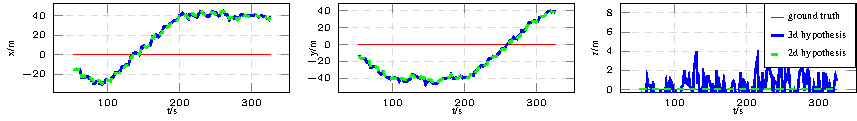
\includegraphics[width=1.0\textwidth]{./fig/plots/example_plot/hypotheses.pdf}
  \caption{Example of a 2D plot using \emph{PGFPlots}.}
  \label{fig:pgfplots_data}
\end{figure}

\section{3D Plots with Sketch}

\emph{Sketch} is a tool for defining a 3D scene using simple descriptive language.
The 3D scene is then converted to \emph{Tikz}, which is later compiled to pdf.
The benefits of using \emph{Sketch} are similar to using \emph{Tikz}: LaTeX fonts, versioning using git, and cleanness of the result.
See the example image in \reffig{fig:coordinate_systems}.
\begin{itemize}
  \item Documentation and manual: \url{http://www.frontiernet.net/~eugene.ressler/}
  \item Cross-compilation from \emph{Sketch} to \emph{pdf} using the \texttt{fig/sketch/compile\_sketch.sh} script.
\end{itemize}

\begin{figure}[htbp]
  \centering
  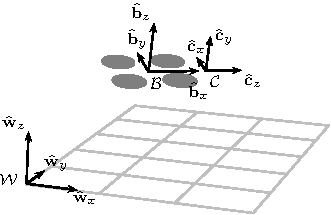
\includegraphics[width=0.4\textwidth]{./fig/sketch/coordinate_frames.pdf}
  \caption{Depiction of the used coordinate systems. The image was drawn using \emph{Sketch}.}
  \label{fig:coordinate_systems}
\end{figure}

\section{Image collages with Subfig}

We recommend using the \texttt{subfig} package, which provides the \texttt{\textbackslash{}subfloat} command.
It is more versatile than the simpler \texttt{subcaption} package.
Check \reffig{fig:uavs} for an example.

\begin{figure}[htbp]
  \centering
  \subfloat[A UAV, the T650 model.] {
    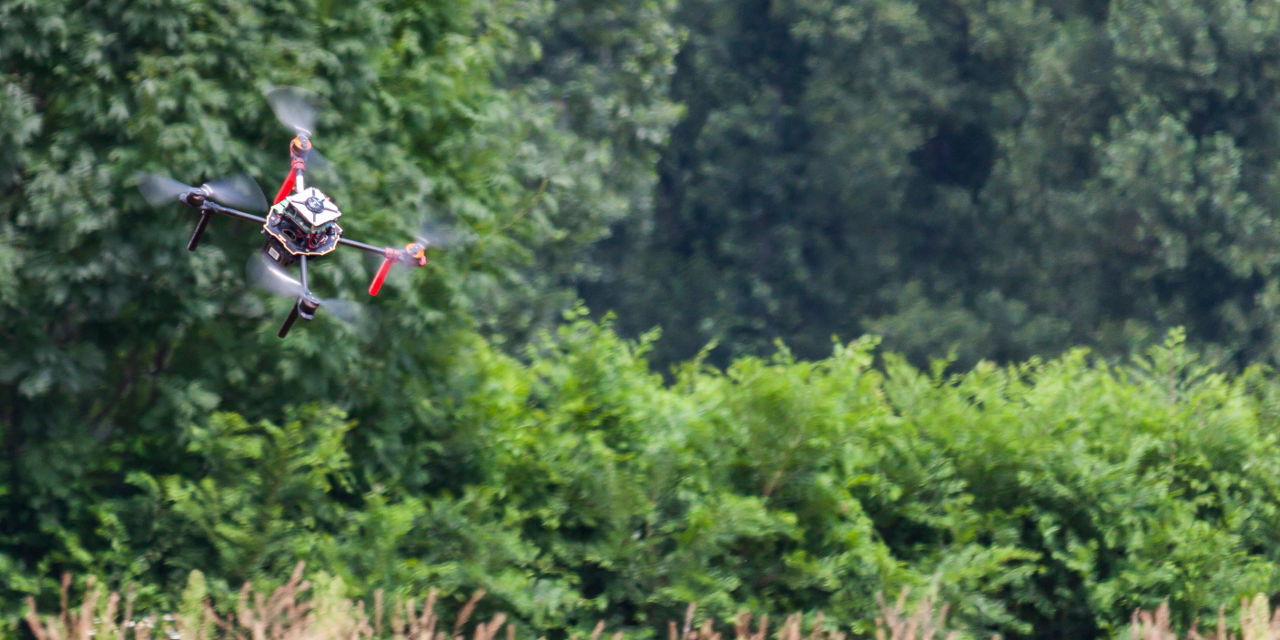
\includegraphics[width=0.48\textwidth]{./fig/photos/uav1.jpg}
    \label{fig:uavs_1}
  }
  \subfloat[Another UAV, again, the T650 model.] {
    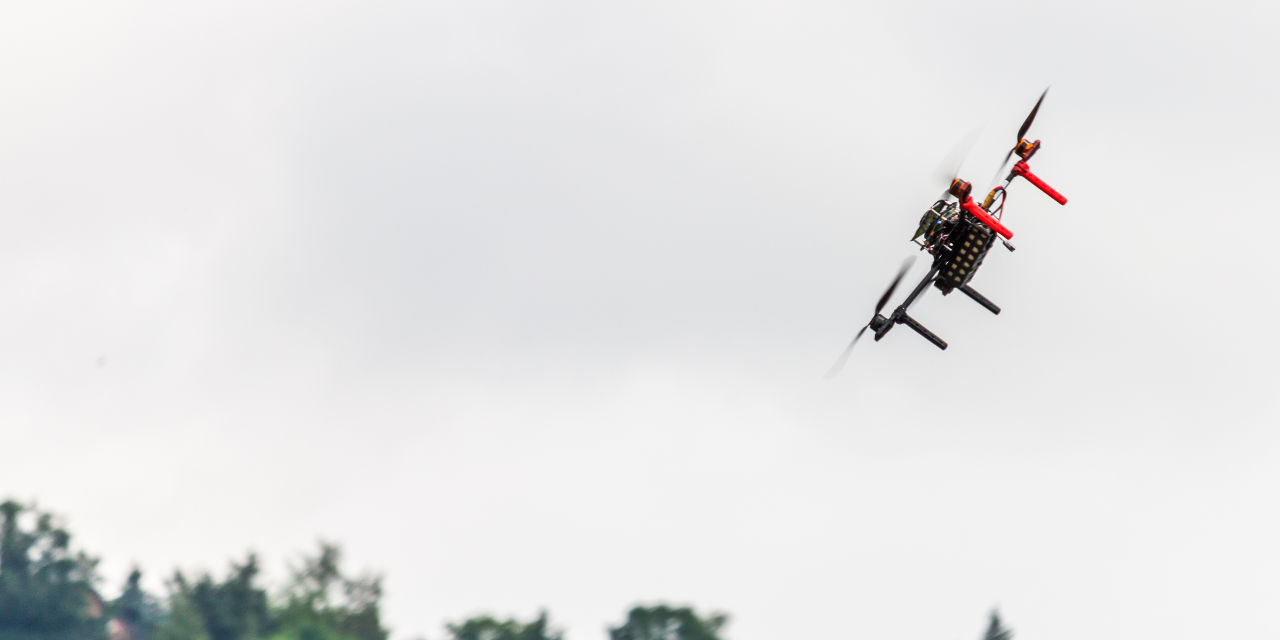
\includegraphics[width=0.48\textwidth]{./fig/photos/uav2.jpg}
    \label{fig:uavs_2}
  }
  \caption{
The caption should mention both subfigures, the \reffig{fig:uavs_1} and the \reffig{fig:uavs_2}.
You can just refer to them as (a) and (b) in the main Figure's caption, but beware, you need to keep it correct as you edit.
}
  \label{fig:uavs}
\end{figure}

\section{Citations with Biblatex}

\emph{Biblatex} is probably the most powerful citation package for LaTeX.
It consumes the standard \texttt{.bib} file. However, it can sort and filter the citations using the \texttt{keywords} tag.
Citing references is done using the \texttt{cite} command, e.g., \cite{baca2021mrs}.
You can also define some nice citation boxes, such as this one:
\fullciteinbox{baca2021mrs}{}

\section{Image overlays with Tikz}

\emph{Tikz} is very useful to create custom image overlays.
The overlay can be set such that the image is spanned by Cartesian coordinates $\left(x, y\right) \in \left[0, 1\right]^2$
Example can be seen in \reffig{fig:tikz_overlay}.

\begin{figure}[!t]

  \centering

  \subfloat {\begin{tikzpicture}
    \node[anchor=south west,inner sep=0] (a) at (0,0) { 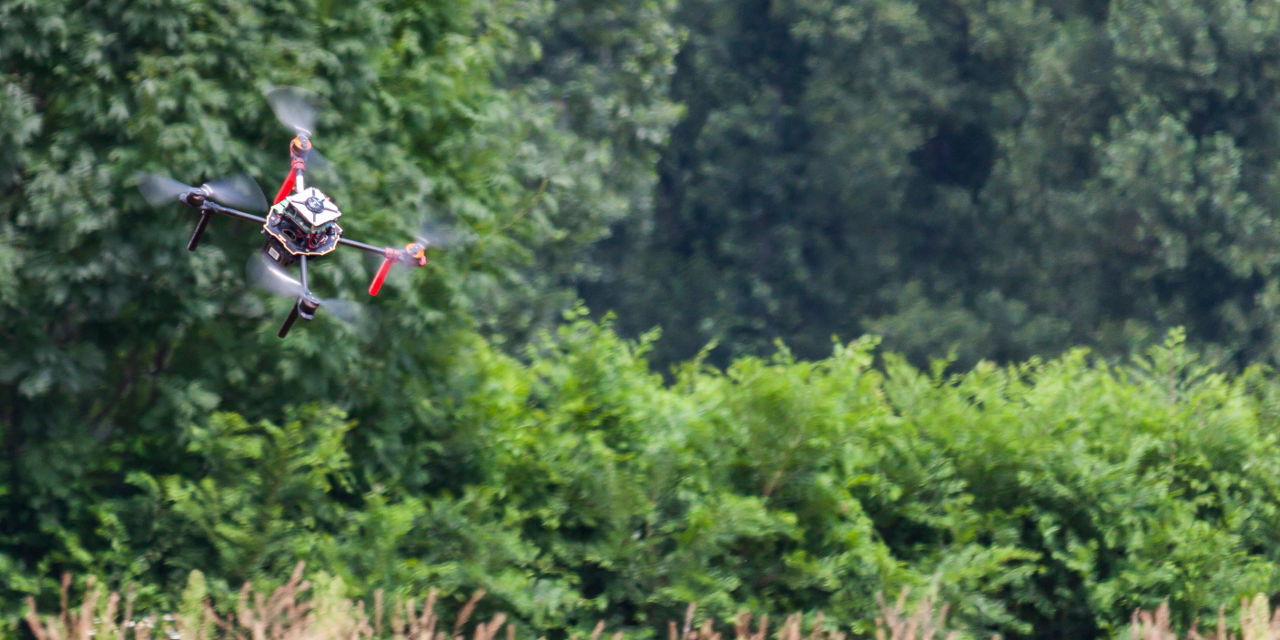
\includegraphics[width=0.45\textwidth]{./fig/photos/uav1.jpg}};
    \begin{scope}[x={(a.south east)},y={(a.north west)}]

      %%{ grid for placing the elements

      % % useful grid to help you find coordinates for plotting the overlay
      % \draw[black, xstep=.1, ystep=.1] (0,0) grid (1,1);
      % \foreach \i in {0,0.1,0.2,0.3,0.4,0.5,0.6,0.7,0.8,0.9,1} {
      %   \node[align=center] at (\i, -0.05) {\i};
      %   \node[align=center] at (\i, 1.05) {\i};
      %   \node[align=center] at (-0.05, \i) {\i};
      %   \node[align=center] at (1.05, \i) {\i};
      % }

      %%}

      % plot some stuff over the image

      % plot white background behind the letter (a)
      \fill[white] (0.001, 0.001) rectangle (0.08,0.14);

      % plot black border
      \fill[draw=black, draw opacity=0.5, fill opacity=0] (0,0) rectangle (1, 1);

      % write the letter (a) in the bottom-left corner
      \draw (0.04,0.06) node [text=black] {\small (a)};

      % plot black border
      \draw[->, white, thick] (0.50, 0.80) -- (0.30, 0.67);
      \draw (0.50,0.86) node [text=white] {\small \textbf{UAV}};
    \end{scope}
  \end{tikzpicture}}
\hfill%
\subfloat {\begin{tikzpicture}
    \node[anchor=south west,inner sep=0] (a) at (0,0) { 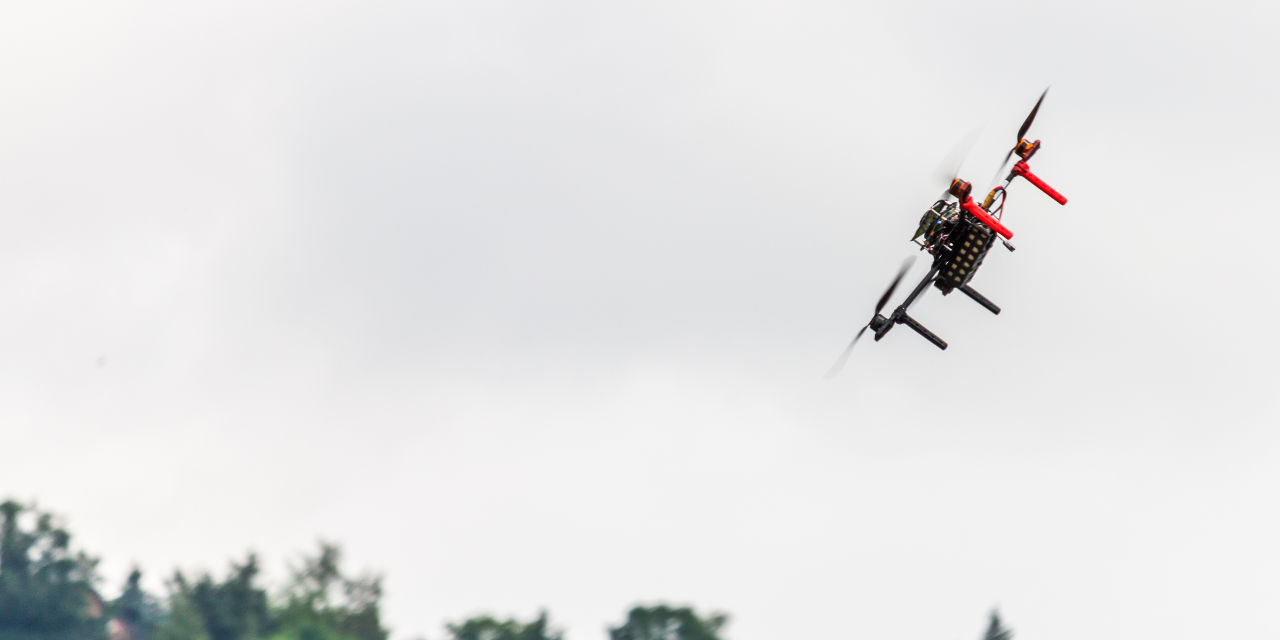
\includegraphics[width=0.45\textwidth]{./fig/photos/uav2.jpg}};
    \begin{scope}[x={(a.south east)},y={(a.north west)}]

      %%{ grid for placing the elements

      % useful grid to help you find coordinates for plotting the overlay
      \draw[black, xstep=.1, ystep=.1] (0,0) grid (1,1);
      \foreach \i in {0,0.1,0.2,0.3,0.4,0.5,0.6,0.7,0.8,0.9,1} {
        \node[align=center] at (\i, -0.05) {\i};
        \node[align=center] at (\i, 1.05) {\i};
        \node[align=center] at (-0.05, \i) {\i};
        \node[align=center] at (1.05, \i) {\i};
      }

      %%}

      % plot some stuff over the image

      % plot white background behind the letter (b)
      \fill[white] (0.001, 0.001) rectangle (0.08,0.14);

      % plot black border
      \fill[draw=black, draw opacity=0.5, fill opacity=0] (0,0) rectangle (1, 1);

      % write the letter (b) in the bottom-left corner
      \draw (0.04,0.06) node [text=black] {\small (b)};
    \end{scope}
  \end{tikzpicture}}


  \caption{Example of using Tikz for image overlays. (a) shows a final product, (b) shows a grid useful for nailing down the coordinates.}
  \label{fig:tikz_overlay}

\end{figure}

\section{General tips}

In general, strive to make the paper easy to read and understand, and hard to misunderstand or misinterpret.
Here are some more specific tips on how to achieve that (and other general suggestions).

\begin{itemize}
  \item
    \textbf{Be consistent.}
    This applies in all contexts.
    For example, if you decide to use the name \enquote{LiDAR}, do not mix it with \enquote{LIDAR} or \enquote{Lidar},
    do not mix different mathematical notations,
    ensure your Figures have the same style and use the same graphics for the same concepts,
    etc.
  \item 
    After you finish writing or modifying any of:
    \begin{itemize}
      \item a sentence,
      \item a paragraph,
      \item a section/chapter,
      \item the whole paper/thesis,
    \end{itemize}
    \textbf{re-read it} to make sure that it makes sense, it is coherent and correct, and doesn't contain typos.
  \item
    If you're using a LLM-based tool (ChatGPT etc.) for grammar-proofing or even formulation of sentences, \textbf{do not just copy-paste its response} to your query.
    The previous rule applies doubly here.
    LLMs tend to often produce confident-sounding nonsense, sentences with reformulated duplicated content, or with a slightly changed meaning.
    They are a good tool to get inspiration to start writing about a subject, for grammar-checking, or for finding alternative, nice-sounding formulations, but they can lie or warp facts --- take care when using them!

\end{itemize}


%% --------------------------------------------------------------
%% |                         Conclusion                         |
%% --------------------------------------------------------------

%!TEX root = ../main.tex

\chapter{Conclusion\label{chap:conclusion_p}}

Summarize the achieved results.
Can be similar as an abstract or an introduction, however, it should be written in past tense.


%% --------------------------------------------------------------
%% |                         References                         |
%% --------------------------------------------------------------

\chapter{References}

\printbibliography[heading=none,title={}]

%% --------------------------------------------------------------
%% |                         Appendices                         |
%% --------------------------------------------------------------

\appendix
\renewcommand\chaptername{Appendix}

\renewcommand{\thechapter}{A}
\renewcommand\chaptername{Appendix A}

\chapter{Appendix A}

\end{document}
